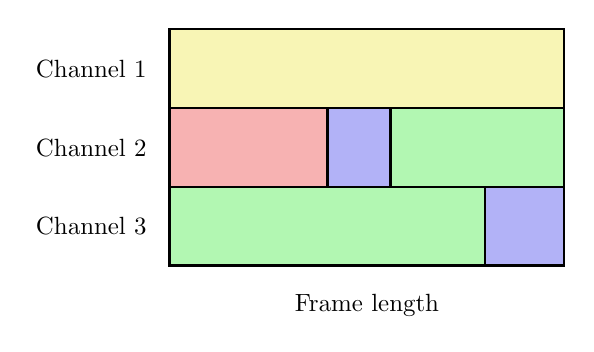
\begin{tikzpicture}
\draw[black,very thick] (-4,-1) rectangle (1,0);
\draw[black,very thick] (-4,0) rectangle (1,1);
\draw[black,very thick] (-4,1) rectangle (1,2);
\draw [step=.3, thick, draw= black, fill=black!10!green!30] (-4,-1) rectangle  (0,0);
\draw [step=.3, thick, draw= black, fill=black!10!blue!30] (0,-1) rectangle  (1,0);
\draw [step=.3, thick, draw= black, fill=black!10!red!30] (-4,0) rectangle  (-2,1);
\draw [step=.3, thick, draw= black, fill=black!10!blue!30] (-2,0) rectangle  (-1.2,1);
\draw [step=.3, thick, draw= black, fill=black!10!green!30] (-1.2,0) rectangle  (1,1);
\draw [step=.3, thick, draw= black, fill=black!10!yellow!30] (-4,1) rectangle  (1,2);
\node[align=center, scale =0.9] at (-1.5,-1.5) {Frame length};
\node[align=center, scale =0.9] at (-5,-.5) {Channel 3};
\node[align=center, scale =0.9] at (-5,.5) {Channel 2};
\node[align=center, scale =0.9] at (-5,1.5) {Channel 1};
\end{tikzpicture}
